%!TEX root = ../thesis.tex

\section{ IMPLEMENTATION }
\subsection{ Data Pre-processing }
The work started by preparing the data so servers could work with it the most efficient way. This
section is devoted to the description of the initial data and how it was processed. The section
also involves comparison of deferent approaches of data structuring, their comparison and
summarizing of the results.

\subsubsection{ Description of the Raw Data }
The provided original data is collected using Google Directions API~\cite{google:directions}
applying following algorithm. First, on top of the city the grid of points was constructed
using WGS~84~\cite{wiki:wgs} coordinate system. Second, for every pair of points the
directions were calculated using HTTP request to the API. Returned data is encoded in JSON
format written to a text file. As result raw data is a
text file where every line is a JSON object received from Google Directions API. The process
of data collection is demonstrated on Figure~\ref{pic:collecting_data}.

\begin{figure}[h]
  \centering
  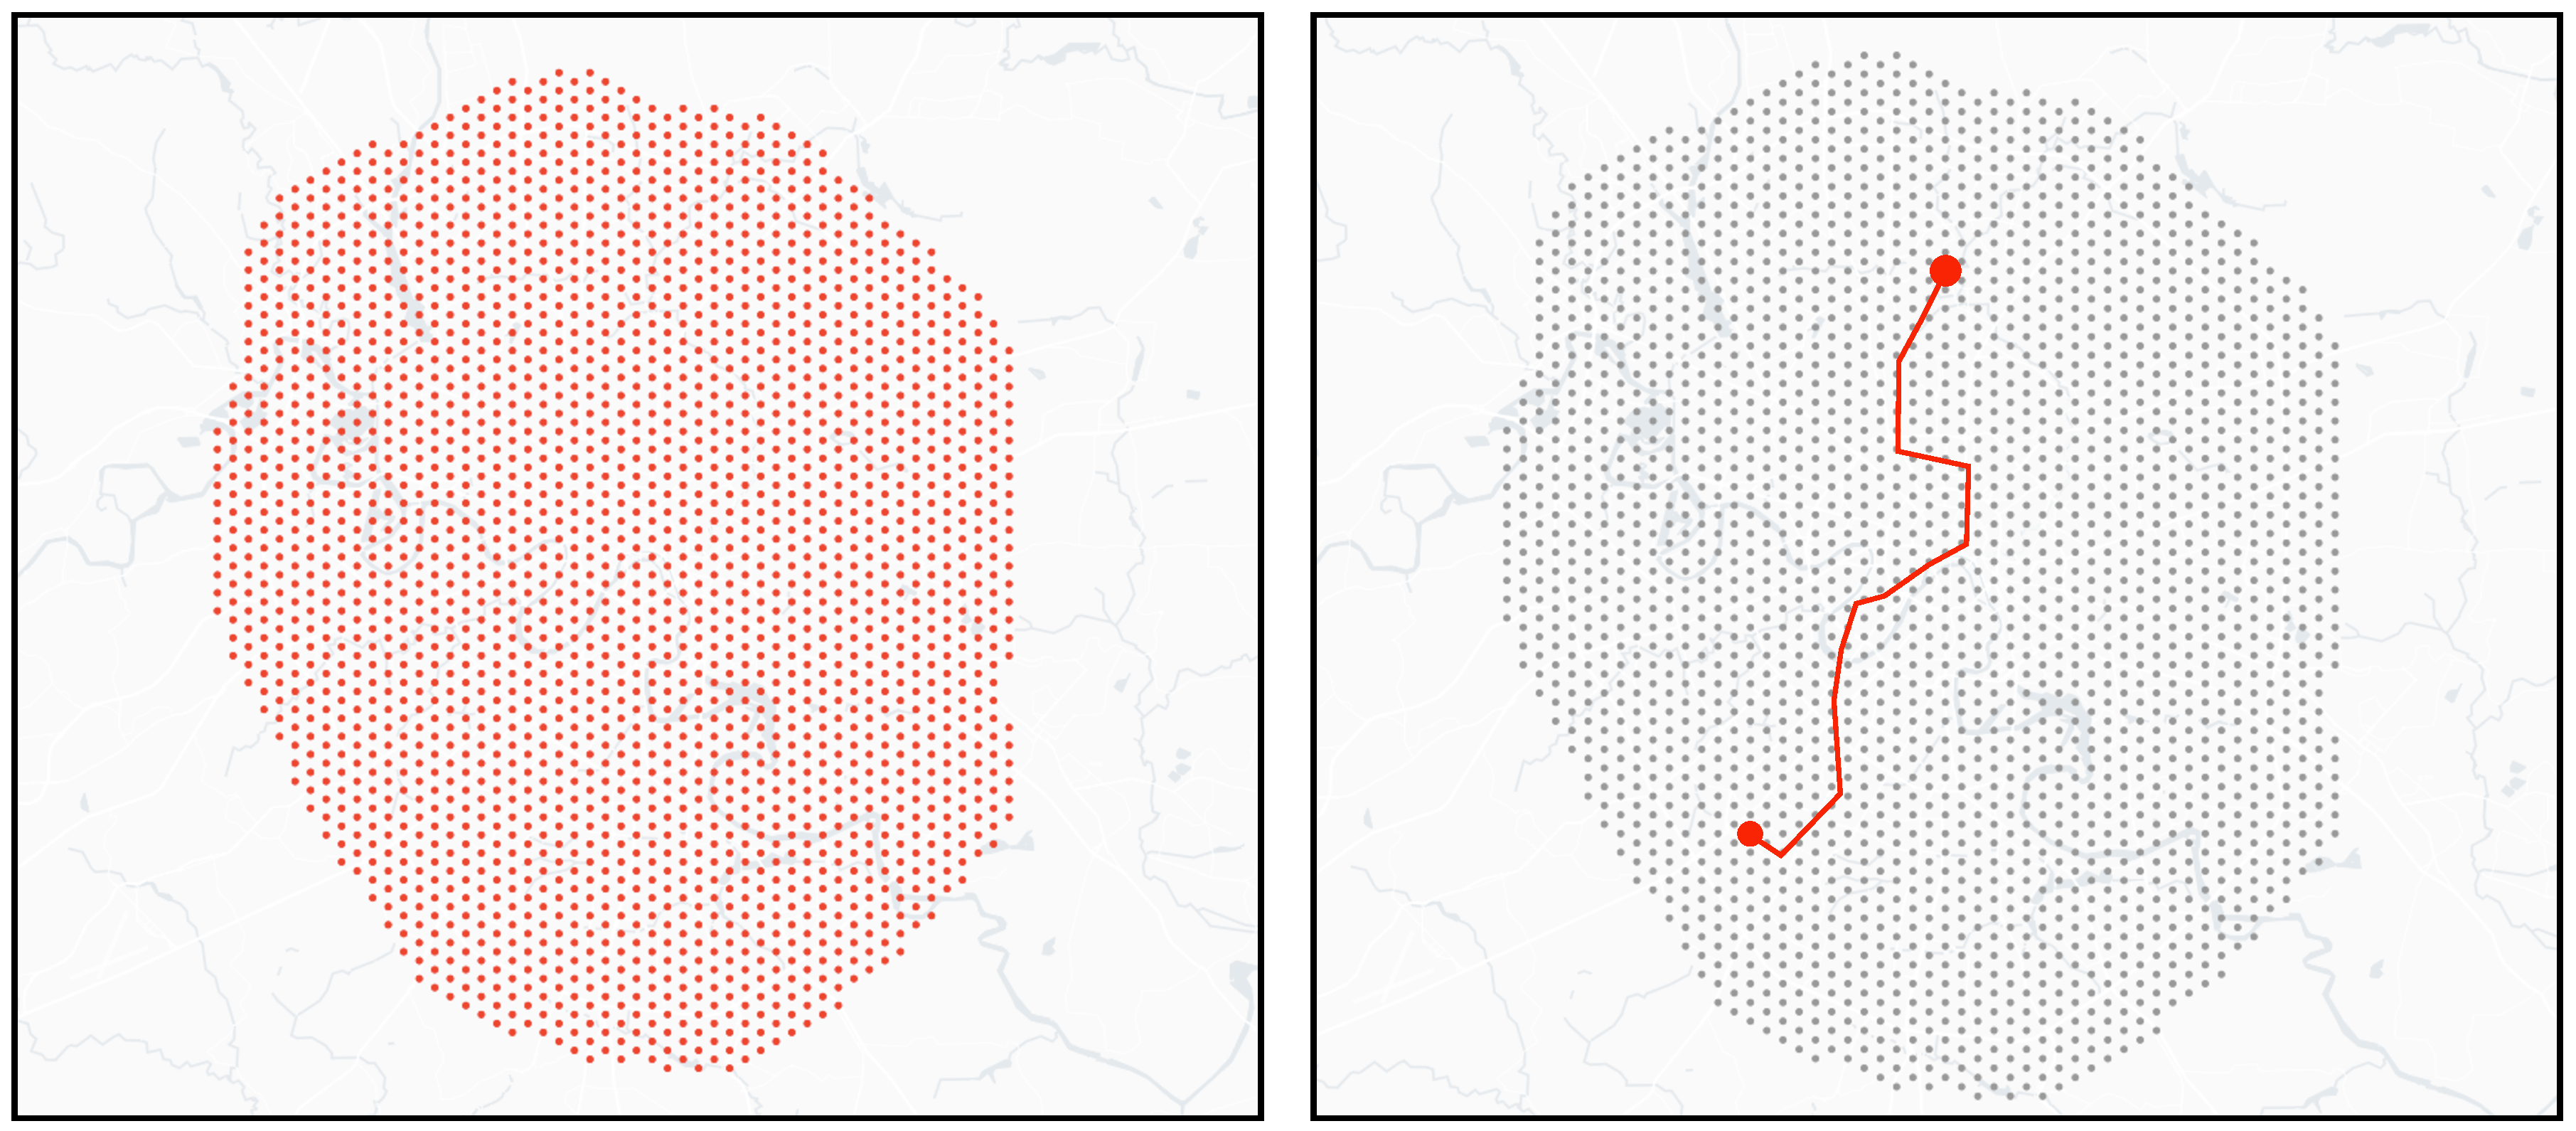
\includegraphics[width=1\textwidth]{data-collection.pdf}
  \caption{The process of the collecting data.}
  \label{pic:collecting_data}
\end{figure}

In fact there is also meta information such as object id, job status, waypoints order,
warnings, but if we simplify and leave only important fields that we will need in pre-processing
step, then JSON object could look like this:

\begin{lstlisting}[language=json, caption=Google Directions API simplified response example,
      label={lst:google_response}]
{
  "start_lat": 55.726497,
  "start_long": 37.338183,
  "end_lat": 55.886619,
  "end_long": 37.579683,
  "data": {
    "routes": [{
      "legs": [{
        "distance": { "text": "45.1 km", "value": 45093 },
        "end_address": "Novgorodskaya ulitsa...",
        "start_address": "Razdorovskaya, Romashkovo...",
        "steps": [{
          "travel_mode": "DRIVING",
          "polyline": { "points": "wicsI{u{bFs@rDC" },
          "distance": { "text": "4.2 km", "value": 4166 },
          "duration": { "text": "7 mins", "value": 438 }
        }, ... ]
      }, ... ]
    }, ... ]
  }
}
\end{lstlisting}

As been be seen from simplified response example, the object contains coordinates of the
start and end point, array routes which consists of \texttt{legs}. \texttt{Legs} are parts of the
route between waypoints. Since in our queries we do not have middle waypoints, the routes array will have
only one element in all cases. Each leg contains total distance information about start and end
location. Also inside \texttt{legs} there is \texttt{steps}, each step is a part of route
which can be described by single command and type of transport, for example ``move forward by bus''
is clearly a step. Step keeps information about its distance and duration which will be needed
to complete this step. Other important things are \texttt{travel\_mode} which indicates what
type of transport is used in this step and \texttt{polyline} which is essentially a set points
of points encoded using lossy Google's algorithm which converts array of float numbers first
to binary representation, then to decimal integers and finally to string using ASCII
codes~\cite{google:polyline}.

\subsubsection{ Extracting Points }

The data collection was initiated before by Mathrioshka, thus the first task was extracting
grid points from the raw data. This step was performed utilizing script written in Python, which
is reading file line by line and extracting starting location point from the data. The
idea of the algorithm is presented in Listing~\ref{lst:points_extraction}. As can be seen from
the listing, Geohash~\cite{wiki:geohash} standard was used to prevent repetitions of the points.
Thus, coordinates could be mapped to strings which can be utilized as ids in points dictionary.
In our implementation for encoding \lstinline{python-geohash} library was used~\cite{pip:geohash}.

\begin{lstlisting}[language=python, caption=Points extraction, label={lst:points_extraction}]
points = []

for line in jsonfile:
    json_obj = json.loads(line)
    slat = json_obj['start_lat']
    slng = json_obj['start_long']
    point = {
        'point_id': geohash.encode(slat, slng),
        'lat': slat,
        'lng': slng
    }
    points[point['point_id']] = point
\end{lstlisting}

\subsubsection{ Extracting Lines }

The second main task was to extract lines from the file, but first to make experiments faster
it was decided to convert data to more convenient format so it would be easier to
experiment with data and process more effectively. Once we have data extracted we will convert it
to the set of GeoJSON files and after that generate vector tiles which will be served by our
tile server.

For intermediate lines representation the CSV file format was selected, due to its simplicity
and availability of the encoders and decoders inside standard Python library. The algorithm is
presented in Listing~\ref{lst:lines_conversion}. First, we initialize table of lines which will
contain all unique lines encoded in raw data. Second, we read file object by object. Each object
is then decomposed into set of lines using \lstinline|lines_from_json()| function. Once lines are
extracted the assertion is performed to check whether the line was already met before. If the
answer is no, then we initialize line, otherwise we just sum distance and duration
and increase weight by one. The distance, duration and weight are necessary to compute
line width, speed, prevailing transport and accessibility of the point.

\begin{lstlisting}[language=python, caption=Lines conversion., label={lst:lines_conversion}]
# Table of lines
T = {}

with open(DATA_PATH) as jsonfile:

    for json_str in jsonfile:
        json_obj = json.loads(json_str)

        for line in lines_from_json(json_obj):
            line_hash = line['line_hash']

            if line_hash not in T:
                del line['line_hash']
                T[line_hash] = line
                T[line_hash]['line_id'] = len(T)
            else:
                T[line_hash]['weight'] += 1
                T[line_hash]['distance'] += line['distance']
                T[line_hash]['duration'] += line['duration']
\end{lstlisting}


